\chapter{Polarization across Dielectric Interface}\label{lec:lec33}
In the last lectures, we have been investigating the behaviour of uniform plane wave across a dielectric media. We studied two cases which are the parallel and perpendicular polarization, and we saw the transmission and reflection across the dielectric boundary. We investigated a special case called total internal reflection across the dielectric boundary. Now we are going to discuss \textbf{polarization across the dielectric interface}. 

If We take a wave which is arbitrarily polarized i.e. the electric field vector makes an arbitrary angle with the plane of incidence and it might also be varying as a function of time. We then see how this behaviour changes when the wave is reflected from the dielectric interface. So what we are going to investigate now is that if the incoming wave is coming with a certain polarization, what will be the polarization of the reflected wave and what will also be the polarization of the transmitted wave?

Any arbitrary state of polarization can be decomposed into two orthogonal polarizations. In this case, we take linear polarization which is parallel and perpendicular to the plane of incidence. This implies that a polarized wave \textbf{E} can be decomposed into \textbf{E}$_\parallel$\footnote{Parallel component of the polarized wave} \textbf{E}$_\parallel$ and \textbf{E}$_\perp$\footnote{vertical component of the polarized wave} \textbf{E}$_\parallel$ and has a phase difference of e$^{j\phi}$ between \textbf{E}$_\parallel$ and \textbf{E}$_\perp$. So the polarized wave will now be \textbf{E} = \textbf{E}$_\parallel$ + \textbf{E}$_\perp$.e$^{j\phi}$.	
\section{Decomposition of Polarized wave}	
when an incident polarized wave \textbf{E$_i$} comes across a dielectric medium, part of it gets transmitted through the media \textbf{E$_t$}, while the rest gets reflected \textbf{E$_r$}, while the rest gets reflected \textbf{E$_r$}. Each of the different parts of the wave i.e. \textbf{E$_i$}, \textbf{E$_t$} and \textbf{E$_r$} can be decomposed into their orthogonal components as explained above.	
\subsection{Incident wave}	
An incident polarized wave \textbf{E$_i$} can be decomposed into two orthogonal components as shown in equation (33.1)	
\begin{equation}
\textbf{E}_i = \textbf{E}_{i\parallel} + \textbf{E}_{i\perp} e^{j\phi}
\end{equation}
figure~\ref{fig:mcben} shows how the incident polarized wave is been decomposed.	
\subsection{Reflected Wave}
A reflected polarized wave \textbf{E$_r$} can be decomposed into two orthogonal components as shown in equation~\ref{fig:mcben1}. It can be denoted by the reflection coefficient as shown in equation~\ref{fig:mcben2}
\begin{equation}
\textbf{E}_r = \textbf{E}_{r\parallel} + \textbf{E}_{r\perp} e^{j\phi}
\end{equation}	
\begin{equation}
\textbf{E}_r = \Gamma_\parallel \textbf{E}_{i\parallel} + \Gamma_\perp \textbf{E}_{i\perp} e^{j\phi}
\end{equation}	
figure~\ref{fig:mcben} shows how the reflected polarized wave is been decomposed.

\subsection{Transmitted Wave}
A transmitted polarized wave \textbf{E$_t$} can be decomposed into two orthogonal components as shown in equation (33.4)	
\begin{equation}
\textbf{E}_t = \textbf{E}_{t\parallel} + \textbf{E}_{t\perp} e^{j\phi}
\end{equation}	
\begin{equation}
\textbf{E}_t = \tau_\parallel \textbf{E}_{i\parallel} + \tau_\perp\textbf{E}_{i\perp} e^{j\phi}
\end{equation}	
figure~\ref{fig:mcben} shows how the transmitted polarized wave is been decomposed.	

\subsection{Combination of \textbf{E$_i$}, \textbf{E$_r$} and \textbf{E$_t$}}
In combining the incident wave \textbf{E$_i$}, reflected wave \textbf{E$_r$} and transmitted wave \textbf{E$_t$} we will get a wave structure as that shown in figure~\ref{fig:mcben}	
\begin{figure}[h]
\centering
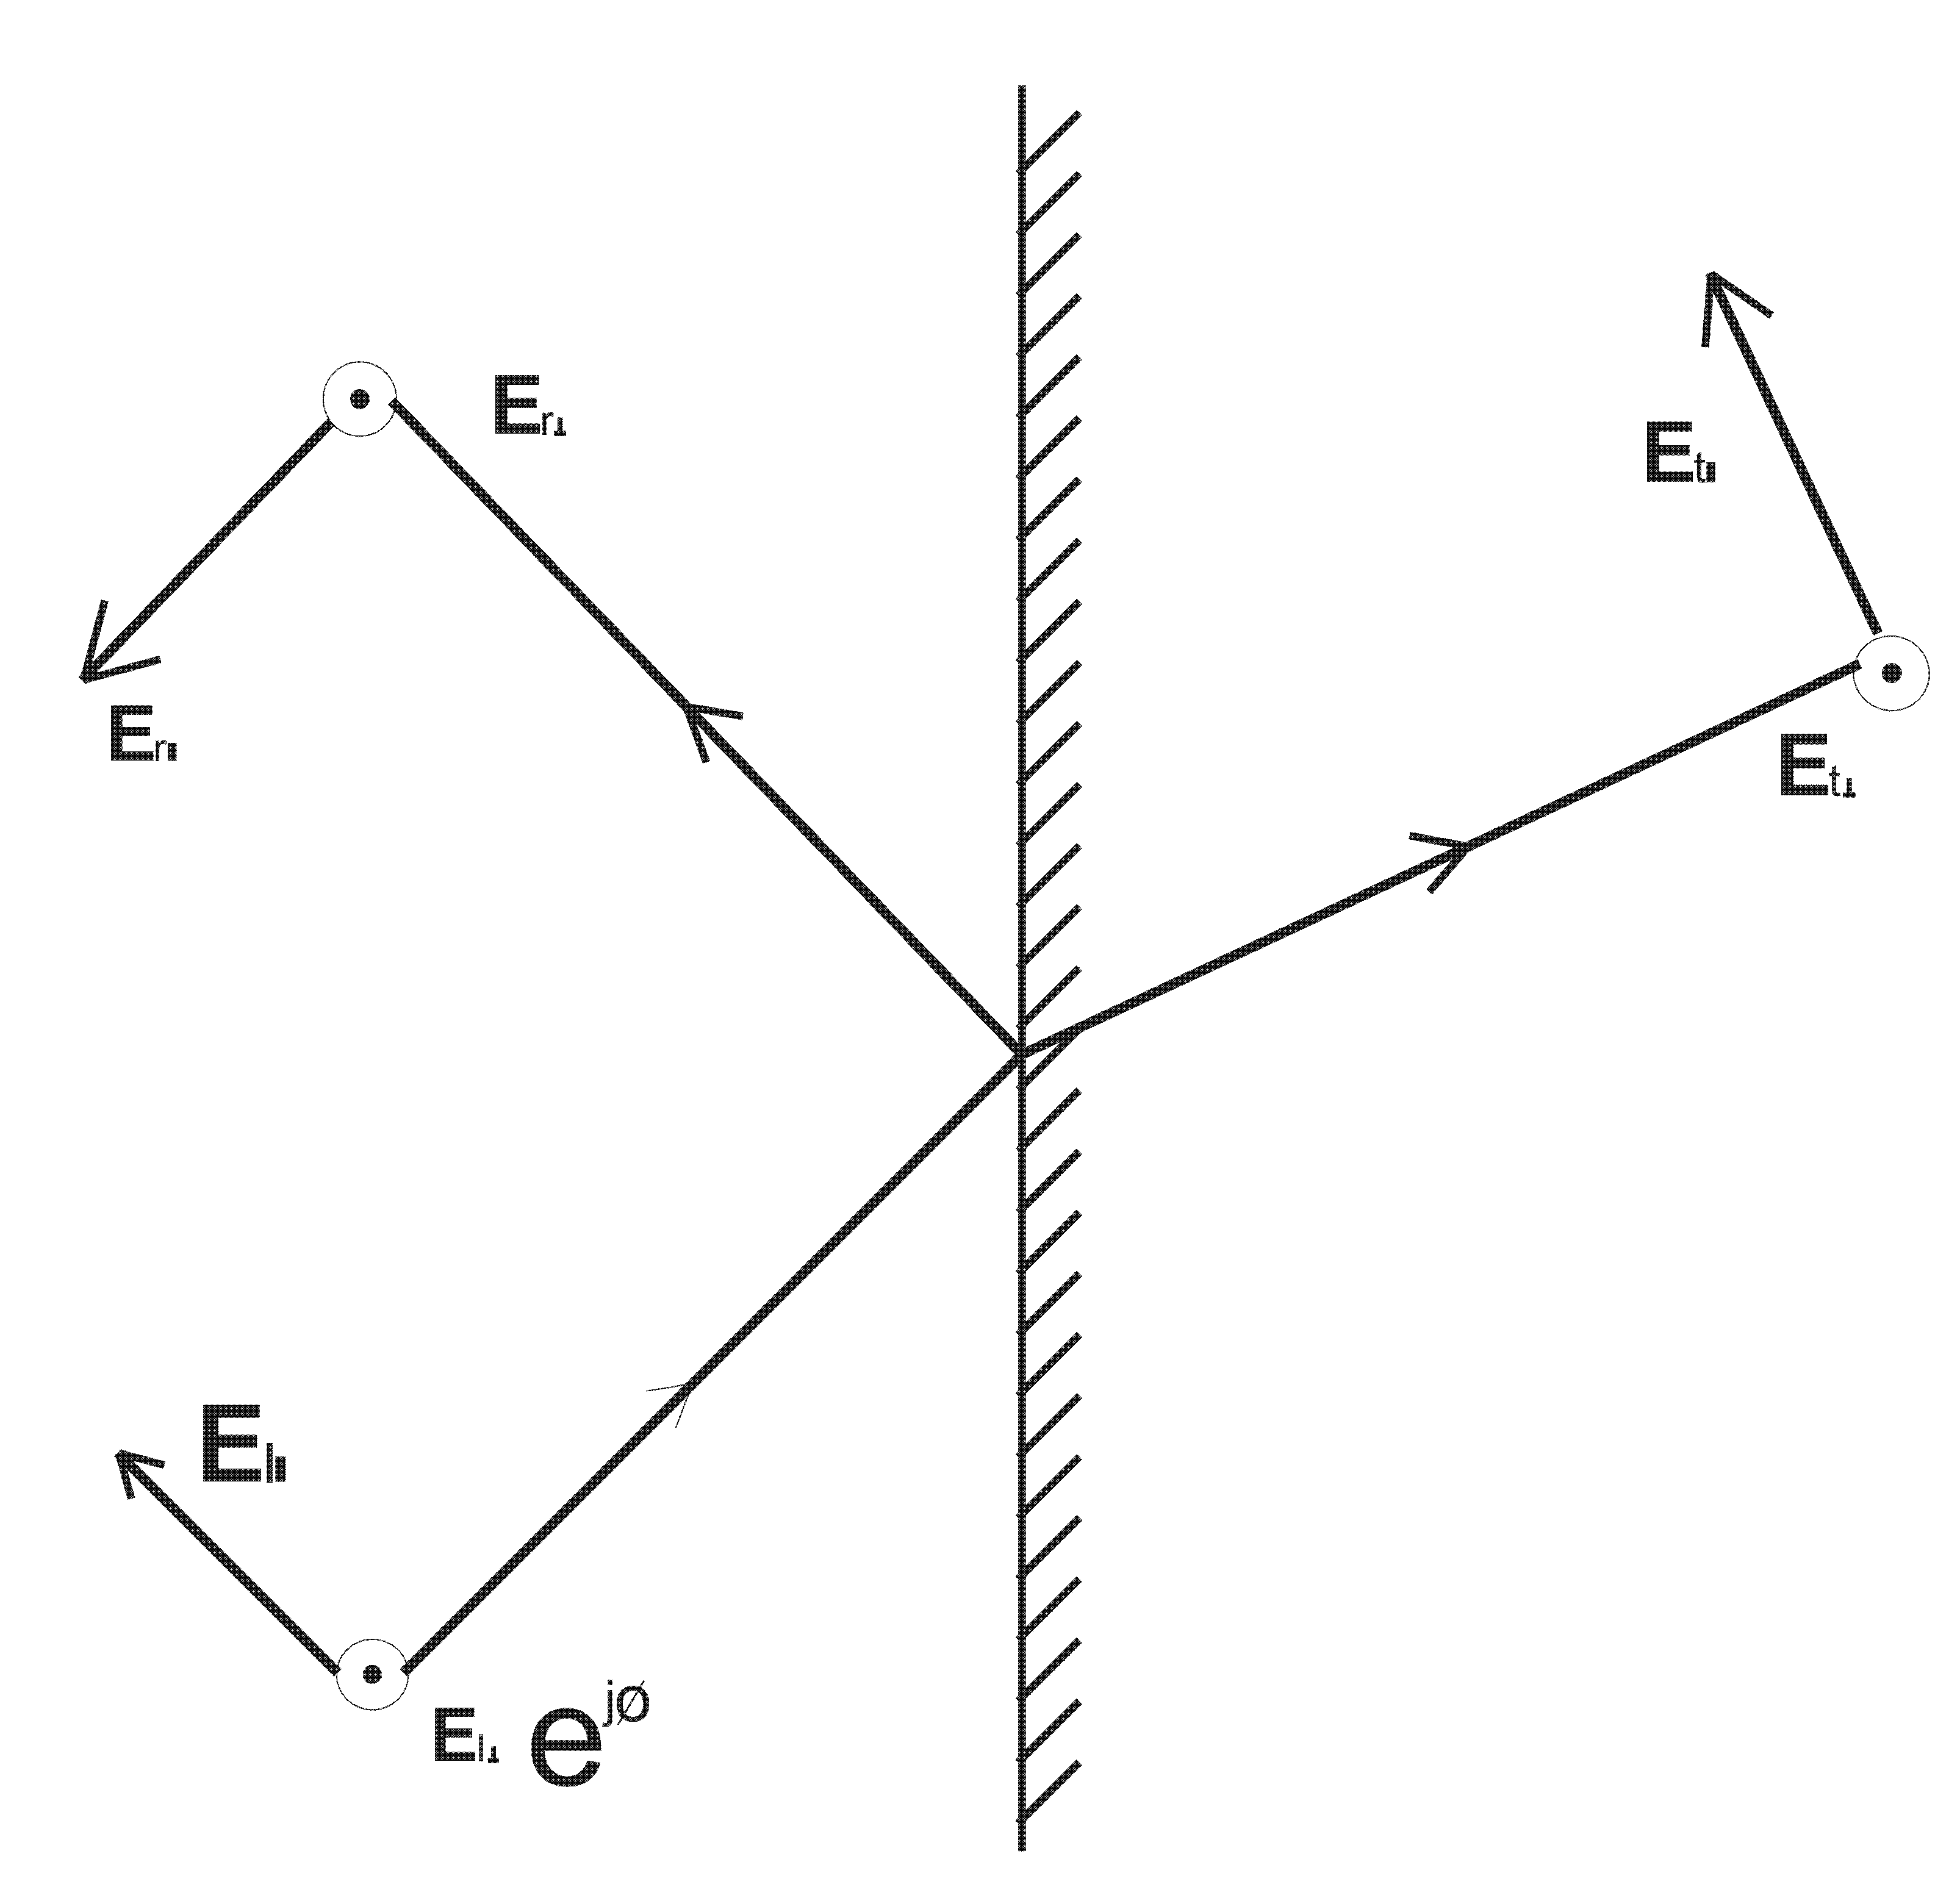
\includegraphics[height=5cm]{\pathtopartone/graphics/mcben}
\caption{Combination of \textbf{E$_i$}, \textbf{E$_r$} and \textbf{E$_t$}}
\label{fig:mcben}
\end{figure}

Depending on whether it is a normal reflection or total internal reflection, $\tau$ and $\Gamma$ could be real or complex quantities. For normal reflection, $\tau$ and $\Gamma$ are real quantities that can have positive or negative. However, for total internal reflection, $\tau$ and $\Gamma$ become complex with a magnitude of one. Now we have various possibilities for special cases which we shall discuss in the next section. <remove>If the wave was linearly polarized and the reflections were normal, what would happen to polarization? If it is a total internal reflection, what would happen to polarization? If the wave was circularly polarized what would happen?

\section{Linearly Polarized Wave}
In a linearly polarized wave, the electric field vector does not change direction as a function of time. That is the incident electric field vector makes an angle with the plane of incidence, but its direction remains the same irrespective of time. A linearly polarized wave can be decomposed into two components that are orthogonal with a phase difference. So if the wave is linearly polarized, the phase difference between \textbf{E}$_{i\parallel}$ and \textbf{E}$_{i\perp}$ is zero. Hence for this case $\phi$ = 0. We shall now investigate what will happen in the case of normal reflection and also in the case of total internal reflection.

\subsection{Normal Reflection}
If $\Gamma_\parallel$ and $\Gamma_\perp$ are real and $\phi$ = 0, then \textbf{E}$_{i\parallel}$ and \textbf{E}$_{i\perp}$ will a phase of 0 or $\pi$ radians between them, depending upon the direction of the electric field. In both cases of 0 or $\pi$ phase difference, the polarization remains linear. Since $\pi$ radians phase shift means a reversal of the electric field. So the orientation of the electric field will change but the polarization will remain linear. So in the general case, $\Gamma_\parallel \neq \Gamma_\perp$. So a linearly polarized wave will remain linearly polarized since phase difference is unchanged, but the relative amplitude for the reflected wave might change depending upon whether $\Gamma_\parallel$ = $\Gamma_\perp$ or $\Gamma_\parallel \neq \Gamma_\perp$. That means the ratio of both components of the reflected wave is not the same as it was for the incident wave. That means the direction of the electric field vector now is changed for the reflected wave. But the wave will remain linearly polarized. So plane of polarization might change depending upon whether $\Gamma_\parallel$ or $\Gamma_\perp$ are equal or not, but the linearly polarized nature of the wave will be maintained.

\subsection{Total Internal Reflection}
On the other hand, if we have total internal reflection, $\Gamma_\parallel$ and $\Gamma_\perp$ are not real, but $\Gamma_\parallel$ = $\Gamma_\perp$ = 1. The phase difference between $\Gamma_\parallel$ and $\Gamma_\perp$ component in the reflected wave will change as $\Gamma_\parallel$ \textbf{E}$_{i\parallel}$ will have its phase and $\Gamma_\perp$ \textbf{E}$_{i\perp}$ e$^{j\phi}$ will have its own phase. So the original phase of $\phi$  = 0 or $\phi$ = $\pi$ radians does not hold here as phase difference between \textbf{E}$_{r\parallel}$  and \textbf{E}$_{r\perp}$ as in normal reflection. So here the phase difference could be arbitrary which means we would get linear polarization changing to elliptic polarization, for the case of total internal reflection. The same thing also applies to the transmitted wave. For normal reflection, a linearly polarized wave remains linearly polarized and elliptic polarization is for total internal reflection.

\section{Circular Polarization}
In a circularly polarized wave,(define circularly polarized wave). So if the incident wave is circularly polarized, what happens to the transmitted and reflected waves at normal reflections and total internal reflection? For circular polarization, $\mid$\textbf{E$_r$$_\parallel$}$\mid$ = $\mid$\textbf{E$_r$$_\perp$}$\mid$ the phase difference between them is $\pm\frac{\pi}{2}$. So $\phi$ = $\pm\frac{\pi}{2}$.

\subsection{Ordinary Reflection}
$\mid\Gamma_\parallel\mid \neq \mid\Gamma_\perp\mid$ but $\Gamma_\parallel$ and $\Gamma_\perp$ are real quantities. That means the phase difference between the reflected wave remains $\phi$ = $\pm\frac{\pi}{2}$. But the amplitude ratio for the reflected wave for perpendicular and parallel are not equal because $\mid\Gamma_\parallel\mid \neq \mid \Gamma_\perp \mid$. So $\mid$ \textbf{E}$_{r\parallel} \mid \neq \mid$ \textbf{E}$_{r\perp\mid}$. But the phase difference between the two remains $\pm\frac{\pi}{2}$. Again the vector sum in this case with varying amplitude gives elliptic polarization. In this case, the major and minor axis align with the coordinate axis for the ellipse. So in this case the incidence wave was circularly polarized. The reflected wave became elliptically polarized. Since the phase difference between these reflected waves is $\frac{\pi}{2}$ radiance still, or ordinary reflection, the major and minor axis of the reflected wave ellipse will lie in the plane of incidence and perpendicular to the plane of incidence respectively or vice versa. But the angle with the major axis makes with the plane of incidence could be either zero or $\frac{\pi}{2}$ radiance. So the tilt angle for the ellipse with respect to the plane of incidence is either 0 or $\frac{\pi}{2}$ radiance.

\subsection{Total Internal Reflection}
With total internal reflection, $\mid\Gamma_\parallel\mid$ = $\mid\Gamma_\perp\mid$ = 1 but $\Gamma_\parallel$ and $\Gamma_\perp$ are complex quantities, meaning
\textbf{E}$_{r\parallel}$ and \textbf{E}$_{r\perp}$ will remain same amplitude with \textbf{E}$_{i\parallel}$ and \textbf{E}$_{i\perp}$ but with different phase which is arbitrary. So we get a wave once again that is elliptically polarized.

In summary, a circularly polarized wave gives at ordinary reflection gives a reflected wave with elliptic polarization with a major axis at 0 or $\dfrac{\pi}{2}$ radians to the phase of incidence (tilt angle) or the case of total internal reflection circularly polarized incident wave gives an elliptically polarized reflected wave.

In general, in an incident wave which is elliptically polarized, the state of polarization of the reflected wave will change depending upon the parameters, an elliptically polarized wave can become circularly polarized or linearly polarized depending upon the medium.

Essentially what we see from the exercise is that the medium interface can be used to alter the state of polarization of the electromagnetic wave. So if we have a certain state of polarization for the incoming wave, then by launching the wave at an arbitrary angle, we should be able to change polarization to the desired state.

One of the special cases to this is that if the incident wave is some arbitrarily polarized wave, is it possible that the reflected wave will be linearly polarized? There are many applications where we require a linearly polarized wave. The source we might have may not generate physically a linearly polarized wave. The source we might have may not generate physically a linearly polarized wave. So we look for some mechanism by which an arbitrarily polarized wave can be converted to a linearly polarized wave. We saw that the dielectric interface can change the polarization of the electromagnetic wave. This could be one of the investigating situations. We investigate if an arbitrary polarization can be converted to a linear polarization.

\section{Brewster Angle}
We recall from earlier lectures that 
\begin{equation}
\Gamma_\parallel = \dfrac{\eta_1\cos\textit{$\theta$i} - \eta_2\cos\textit{$\theta$t}}  {\eta_1\cos\textit{$\theta$i} - \eta_2\cos\textit{$\theta$t}}
\end{equation}
\begin{equation}
\tau_\parallel = \dfrac{2\eta_2\cos\textit{$\theta$i}} {\eta_1\cos\textit{$\theta$i} + \eta_2\cos\textit{$\theta$t}}
\end{equation}
\begin{equation}
\Gamma_\perp = \dfrac{\eta_2\cos\textit{$\theta$i} - \eta_1\cos\textit{$\theta$t}}  {\eta_2\cos\textit{$\theta$i} - \eta_1\cos\textit{$\theta$t}}
\end{equation}
\begin{equation}
\tau_\perp = \dfrac{2\eta_2\cos\textit{$\theta$i}} {\eta_1\cos\textit{$\theta$i} + \eta_2\cos\textit{$\theta$t}}
\end{equation}
We ask if $\eta_1\cos\theta_{\textit{i}}$ - $\eta_2\cos\theta_{\textit{t}}$ = 0  for parallel or $\eta_2\cos\theta_{\textit{i}}$ - $\eta_1\cos\theta_{\textit{t}}$ = 0 for perpendicular polarization i.e $\Gamma$ = 0. Then the wave incident on the dielectric interface is completely transmitted to the second medium. That means if we put a perpendicularly polarized wave at an angle $\Gamma_\perp$ = 0, then the perpendicularly polarized wave goes through without reflection. Similarly a parallel polarized wave incident on the medium with the angle at which $\Gamma_{\parallel}$ = 0, the parallel polarized wave passes through and there is no reflection.
Now if we have an arbitrarily polarized wave and launch at an angle which satisfies $\Gamma_\perp$ = 0, only the perpendicularly polarized component goes through. If it launched at an angle at which $\Gamma_\parallel$ = 0 only the parallel component of polarization pass through the medium. In either case, the reflected wave would have parallel and horizontal polarization for $\Gamma_\parallel$ = 0 and $\Gamma_\perp$ = 0 respectively. In both situations what is transmitted becomes essentially linear polarization. We have now the interesting case that for a given parameter, we look for the angle at which $\Gamma_\parallel$ or $\Gamma_\perp$ goes to zero. At this angle, one of the polarization is reflected, and a complimentary polarization is transmitted to the second medium. So an arbitrary state of polarization can be converted to linear polarization.

For parallel polarization, $\Gamma_\parallel$ = 0 when $\eta_1\cos\theta$i - $\eta_2\cos\theta$t = 0 or $\eta_1\cos\theta$i = $\eta_2\cos\theta$t. For perpendicular polarization $\Gamma_\perp$ = 0 i.e $\eta_2\cos\theta$i - $\eta_1\cos\theta$t = 0 or $\eta_2\cos\theta$i = $\eta_1\cos\theta$t. $\eta_1$ and $\eta_2$ are the intrinsic impedance of medium 1 and 2 respectively. From snell's law $\beta_1\sin\theta$i = $\beta_2\sin\theta$t. The incident angle $\theta_i$ we solve for in the case of parallel and perpendicular polarization, after some algebraic manipulation can be expressed as equations 33.10 and 33.11. 
\begin{equation}
\tan\theta_{B\parallel} = \dfrac{\beta_2}{\eta_2} \Bigg\{ \dfrac{\eta_1 ^2 - \eta_2 ^2}{\beta_1 ^2 - \beta_2 ^2} \Bigg\}^{\dfrac{1}{2}}
\end{equation}
\begin{equation}
\tan\theta_{B\perp} = \dfrac{\beta_2}{\eta_1} \Bigg\{ \dfrac{\eta_2 ^2 - \eta_1 ^2}{\beta_2 ^2 - \beta_1 ^2} \Bigg\}^{\dfrac{1}{2}}
\end{equation}

These angles at which the reflection coefficient goes to zero $\Gamma_\parallel$ = $\Gamma_\perp$ = 0 are called the BREWSTER ANGLE, so therefore $\theta_B$ is the brewster angle. So we have Brewster angle for parallel and perpendicular polarization. In general, if we take a medium which could be magnetic, then the Brewster angle for both polarization exists ($\parallel$ or $\perp$). So at the Brewster angle for parallel polarization, the reflected wave will have only a perpendicularly polarized wave and at the Brewster angle for perpendicular polarization, the reflected wave has only a parallel wave. The angle says for $\tan\theta_{B\parallel}$ Was derived as follows.
\subsection{Parallel Polarization}
previously, we derive the relationships bellow
\begin{dmath}
\eta_1\cos\theta_i = \eta_2\cos\theta_t  = \eta_2\sqrt{1 - \sin^2\theta_t} = \eta_2\sqrt{1- \Bigg\{\dfrac{\beta_1}{\beta_2}\Bigg\}\sin\theta_i}
\end{dmath}
we also have that $\beta_1\sin\theta_i$ = $\beta_2\sin\theta_t$ from snell's law. so
\begin{equation*}
\beta_2\eta_1\cos\theta_i = \eta_2\sqrt{\beta_2^2-\beta_1^2\sin^2\theta_i}
\end{equation*}
or
\begin{equation}
\cos\theta_i\dfrac{\beta_2\eta_1}{\eta_2} = \sqrt{\beta_2^2-\beta_1^2\sin^2\theta_i}
\end{equation}
if we square both sides from equation (33.13), we get
\begin{equation*}
\cos^2\theta_i \dfrac{\beta^2_2\eta^2_1}{\eta^2_2} = \beta^2_2 - \beta^2_1\sin^2\theta_i
\end{equation*}
or
\begin{equation}
\dfrac{\beta^2_2\eta^2_1}{\eta^2_2}(1 - \sin^2\theta_i) = \beta^2_2 - \beta^2_1\sin^2\theta_i
\end{equation}
\begin{equation*}
\dfrac{\beta^2_2\eta^2_1 - \beta^2_2\eta^2_2}{\eta^2_2} = (\dfrac{\beta^2_2\eta^2_1}{\eta^2_2} - \beta^2_1)\sin^2\theta_i
\end{equation*}
\begin{equation*}
\beta^2_2\eta^2_1 - \beta^2_2\eta^2_2 = (\beta^2_2\eta^2_1 - \beta^2_1\eta^2_2)\sin^2_{\theta i}
\end{equation*}
\begin{equation}
\sin^2_{\theta i} = \dfrac{\beta^2_2\eta^2_1 - \beta^2_2\eta^2_2}{\beta^2_2\eta^2_1 - \beta^2_1\eta^2_2}
\end{equation}
from trigonometry, we have that,
\begin{equation*}
\cos^2_{\theta i} = 1 - \sin^2_{\theta i}
\end{equation*}
so substituting that in equation (33.15) we get 
\begin{equation}
\cos^2_{\theta i} = 1 - \Bigg\{\ \dfrac{\beta^2_2\eta^2_1 - \beta^2_2\eta^2_2}{\beta^2_2\eta^2_1 - \beta^2_1\eta^2_2} \Bigg\}
\end{equation}
also from trigonometry, we know that
\begin{equation*}
\tan^2\theta_i = \dfrac{\sin^2\theta_i}{\cos^2\theta_i} = \Bigg\{\ \dfrac{\beta^2_2\eta^2_1 - \beta^2_2\eta^2_2}{\beta^2_2\eta^2_1 - \beta^2_1\eta^2_2} \Bigg\} = \Bigg\{\ \dfrac{\beta^2_2\eta^2_2 - \beta^2_2\eta^2_1}{\beta^2_2\eta^2_1 - \beta^2_1\eta^2_2} \Bigg\}
\end{equation*}
replacing $\theta_i$ with $\theta B_\parallel$
\begin{equation}
\tan\theta_{B\parallel} = \sqrt{\dfrac{\beta^2_2(\eta^2_1 - \eta^2_2)}{\eta^2_2(\beta^2_2 - \beta^2_1)}} = \dfrac{\beta_2}{\eta_2}\Bigg\{\ \dfrac{\eta^2_1 - \eta^2_2}{\beta^2_2 - \beta^2_1} \Bigg\}^{\frac{1}{2}}
\end{equation}

\subsection{Perpendicular Polarization}
Let's assume that the electric field was perpendicular to the plane of incidence as shown in figure~\ref{fig:mcben1} with a dot (arrow pointing outward) i.e. perpendicular to the plane of the paper. irrespective of variation in $\theta_i$, \textbf{E}$_i$ will remain perpendicular to the plane of incidence and its amplitude is fixed. so when the continuity of the electric field is applied, we get a reflected and transmitted field. The sum of \textbf{E}$_i$ and \textbf{E}$_r$ must be equal to \textbf{E}$_t$ i.e tangential component of the electric field must be continuous across the boundary. The amplitude of \textbf{E}$_i$, \textbf{E}$_r$ and \textbf{E}$_t$ don't depend on lunching angle $\theta_i$. Hence the \textbf{E}$_r$ will always be needed to satisfy the boundary condition at the interface.
\begin{figure}[h]
\centering
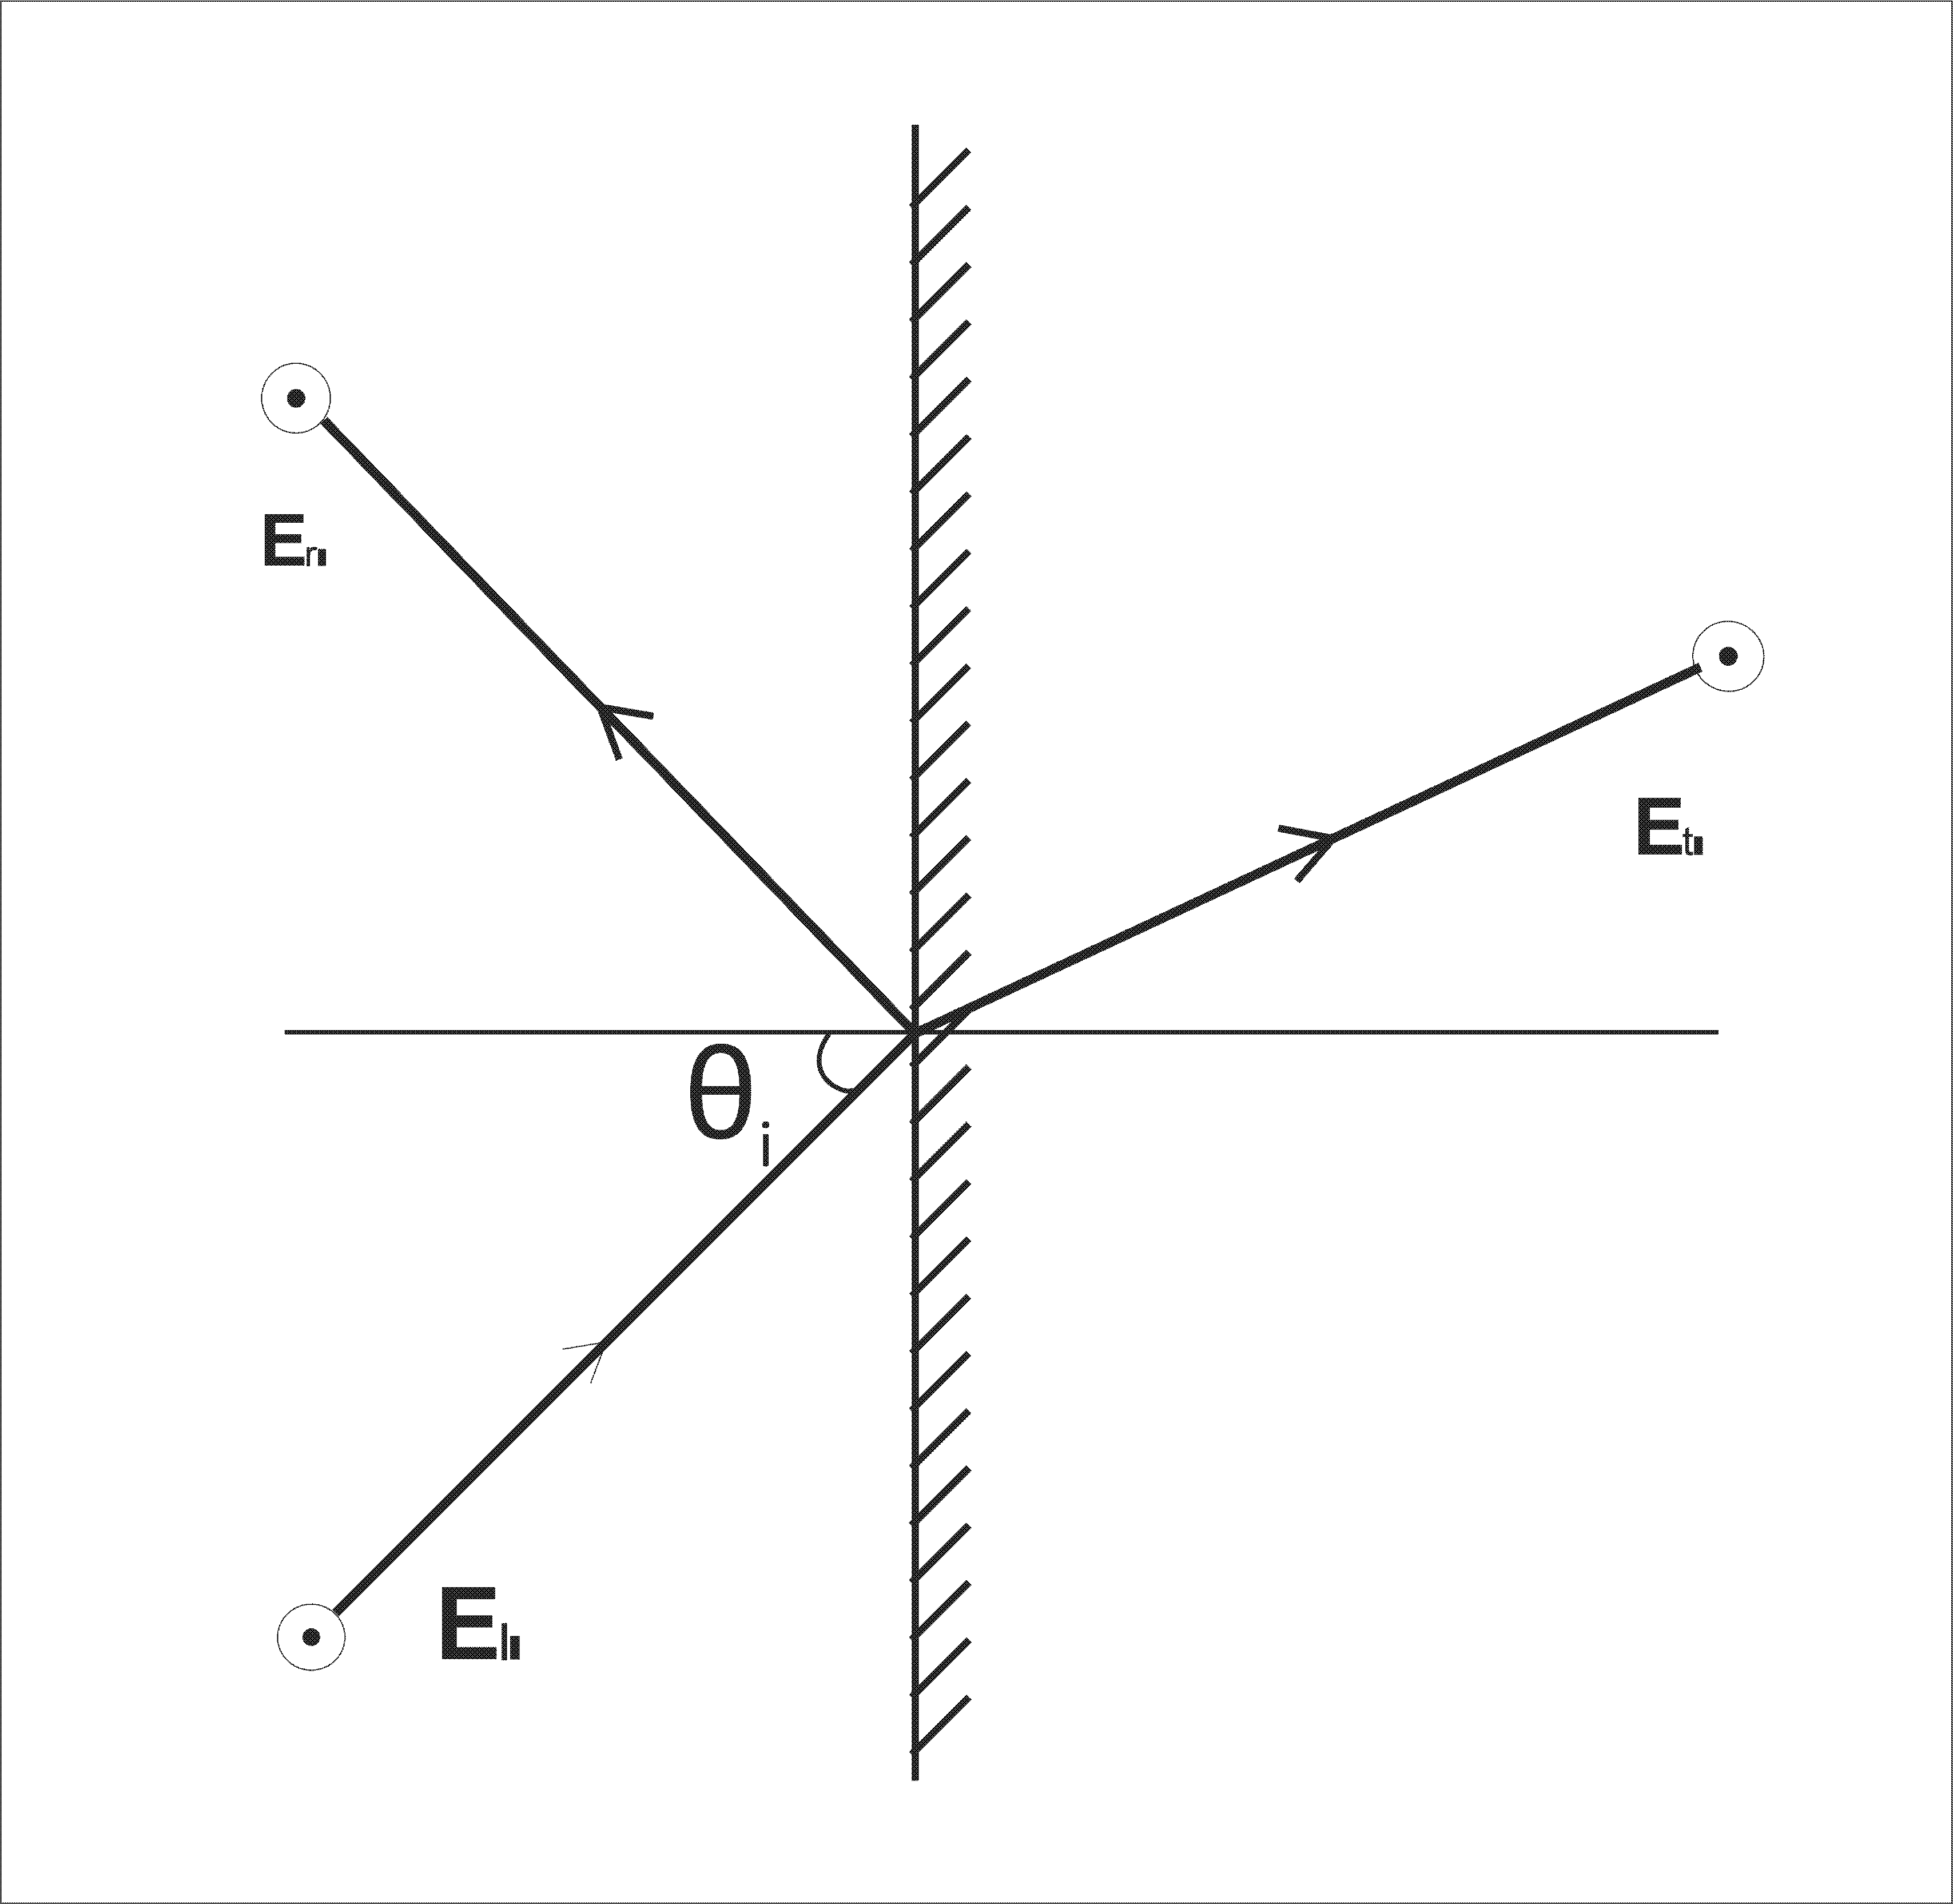
\includegraphics[height=5cm]{\pathtopartone/graphics/mcben1}
\caption{}
\label{fig:mcben1}
\end{figure}
\begin{figure}[h]
\centering
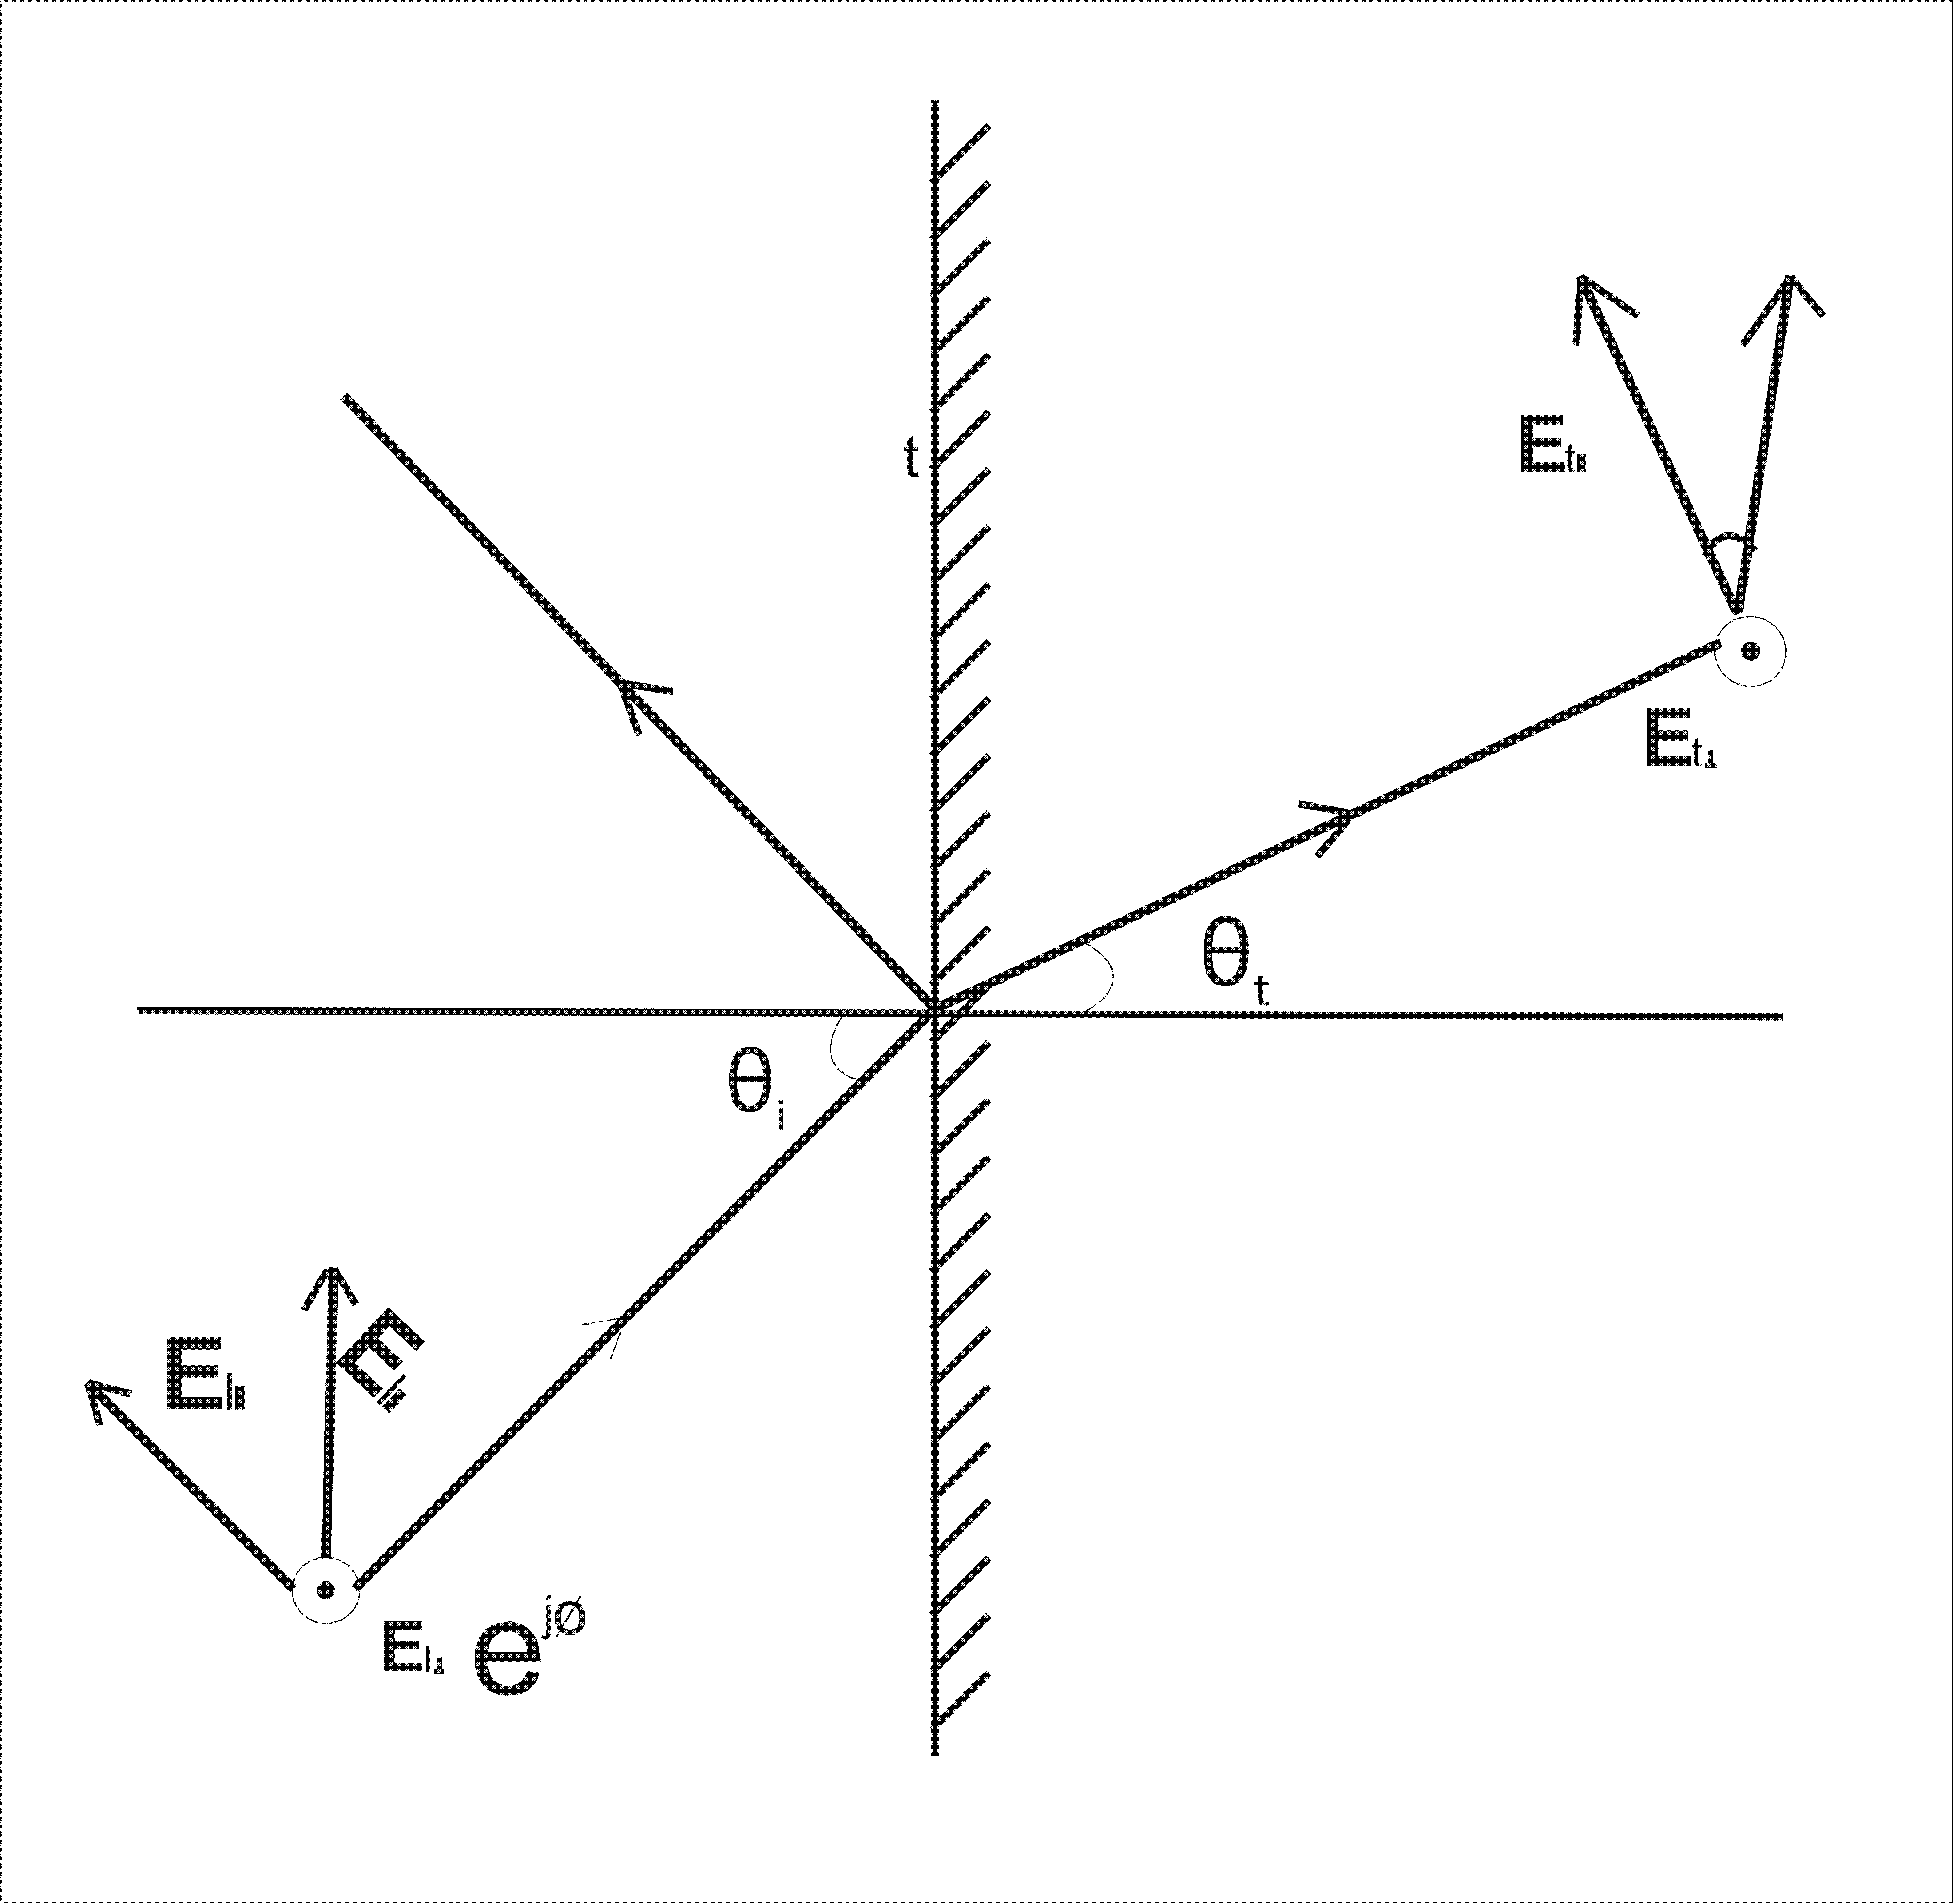
\includegraphics[height=5cm]{\pathtopartone/graphics/mcben2}
\caption{}
\label{fig:mcben2}
\end{figure}	

However for the parallel polarization, variation of $\theta_i$ affects the tangential component of \textbf{E}$_i$ and \textbf{E}$_t$ and they vary with $\theta$ as shown in figure~\ref{fig:mcben2} So there is one angle at which \textbf{E}$_t$ tangential equal to \textbf{E}$_i$ tangential i.e \textbf{E}$_i\cos\theta_i$ = \textbf{E}$_t\cos\theta_t$, then electric field due to reflection is not required any more to satisfy the boundary condition. That means \textbf{E}$_r$ will not be needed anymore to satisfy the boundary condition at the interface. so at \textbf{E}$_i\cos\theta_i$ = \textbf{E}$_t\cos\theta_t$, the wave incident is completely transmitted. Since the tangential component varies as the angle of incidence varies, at some point, there is no reflected electric field required to satisfy the boundary condition.

For perpendicular polarization, this is not the case because the electric field perpendicular to the plane of the paper does not depend on $\theta_i$ and so \textbf{E}$_r$ is always required, so that \textbf{E}$_i$ + \textbf{E}$_r$ = \textbf{E}$_t$. if $\mu_1 \neq \mu_2 \neq \mu_3$ i.e the media were magnetic, so whatever applies to the electric field applies to magnetic fields and then we have brewster angle for perpendicular polarization also. however, for a media with a pure dielectric, the brewster angle will exist for parallel polarization and will not exist for perpendicular polarization. $\theta_{B\parallel}$ = $\tan^{-1}\left(\sqrt{\dfrac{\textbf{E}_2}{\textbf{E}_1}}\right)$ = $\tan^{-1}\left(\dfrac{\eta_2}{\eta_1}\right)$ were $\eta_2$ and $\eta_1$ are refractive index so therefore $\dfrac{\eta_2}{\eta_1}$ = $\sqrt{\dfrac{\textbf{E}_{r2}}{\textbf{E}_{r1}}}$.

Generally, for the dielectric medium, we have the Brewster angle for parallel polarization. One can make use of this Brewster angle for converting an arbitrarily polarized wave to a linearly polarized wave. From the diagram below, the incident wave is arbitrarily polarized hence it would have perpendicular and parallel polarization c. As the incidence angle = $\theta_{B\parallel}$, the reflected wave is made out of purely perpendicular polarization \textbf{E}$_{i\perp}$ as shown by the symbol. For the transmitted wave , the \textbf{E}$_{i\parallel}$ passes through since incidence angle is $\theta_{B\parallel}$. Some of the perpendicular components will pass through also as $\theta_{B\parallel}$ is not its polarizing angle of $\theta_{B\perp}$. Hence it is just like a normal wave incident at an angle. So the transmitted wave can in general be elliptic polarization since it has both $\theta_{B\parallel}$. So without worrying about the state of polarization of the incoming wave, whether linear, circular or elliptically polarized, if the wave is launched at the Brewster angle, then the reflected wave will have a polarization which is linear polarization and its orientation is perpendicular to the plane of incidence. So for any arbitrarily polarized wave, the reflected wave \textbf{E}$_{r\perp}$ points outward in the manner shown perpendicular to the plane of incidence. For this reason $\theta_{B\parallel}$ is called the \textbf{polarizing angle}. Since a wave launched at that angle has a reflected wave which is linearly polarized. The polarizing angle finds application in polarizing the light beams in lasers, ie if the polarization was arbitrary, we can always use the Brewster angle to make sure the reflected wave is linearly polarized. 

So our conclusion from the discussion is that by using the dielectric interfaces, one can change the state of polarization of electromagnetic waves. This is been shown here for optical beams. But for other radio frequencies, one can make use of this phenomenon for changing the state of polarization of electromagnetic waves.
Later in reflection and refraction from conducting boundaries, how the state of polarization would be affected from the incident to the reflected wave?  We have seen for the light incident of Brewster angle, an arbitrary polarization gives a reflected light that is linearly polarized. In conducting boundaries, the case is a little simpler and we will observe an interesting phenomenon then. So this essentially gives us an idea of how to use dielectric boundary to change the state of polarization of electromagnetic waves. 

Suppose we have a general boundary for which $\sigma_1 \neq \sigma_2 \neq 0$ is shown below. We know medium parameters like propagation constant and intrinsic impedances of the media. So we ask what happens to the reflected and transmitted wave in this general media? To solve this problem we first satisfy the boundary condition at the interface. We have satisfied the boundary condition for a tangential component of electric and magnetic fields. If conductivity is not zero, then we have a surface current and because of that, the expression for $\gamma_\parallel$ and $\gamma_\perp$ is still valid. That of $\tau_\parallel$ and $\tau_\perp$ is also valid. But the expression for the intrinsic impedance in both cases $\eta_1$ and $\eta_2$ is now $\eta_1$ = $\sqrt{\dfrac{j\omega\mu_1}{\sigma_1 + j\omega\epsilon_1}}$ and $\eta_2$ = $\sqrt{\dfrac{j\omega\mu_2}{\sigma_2 + j\omega\epsilon_2}}$  and because of this the transmission and reflection coefficient becomes complex quantities.
So a general lossy media like this, the analysis is the same with $\eta_1$ and $\eta_2$ appropriately chosen. But with $\gamma$ = $\alpha + j\beta$ being complex in the presence of loss then FU, with $\gamma$ indicating that there is some attenuation in the system. 

When a plane Wave is an incident on this lossy interface, it does not matter from where the wave originated since the wave amplitude doesn't change even if we travel an infinite distance for a lossless medium. However for a lossy media if we assume that this wave was incident on the boundary at an infinite distance from the surface and $\gamma_1$ = $\alpha_1 + j\beta_1$ ie complex, then the wave amplitude decreases exponentially as it travels. So after travelling a certain distance, the amplitude which reaches the surface or building interface of the lossy media is zero. Similarly, if we had considered that the wave had a finite amplitude at the interface, coming from a distance - $\infty$ as a plane wave, then it should have infinite amplitude from the point where the wave originated. so in the case of a lossy medium, it would look as if we require infinite energy to start with if the wave travels from infinity. This is a hypothetical situation. without getting into the issue of where the media interface has a certain amplitude, we can assume that when the wave reaches the media interface and just after the media interface will be given by the reflection and transmission coefficient respectively. when a wave travels from medium 1 to another medium 2, it will slowly attenuate. the incident wave amplitude is giving as you move away from the interface towards the left of medium 1. so in medium 2, we have a travelling wave with propagation constant $\gamma_2$ and whose amplitude is exponentially decaying as we move in the direction of travel.

In medium 1, the fields seen are a superposition of incident and reflected waves, the incidence wave grows as we go away from the interface. This case is identical to a lossy transmission line. As we go away from the interface or termination point in a transmission line, the reflected wave becomes weaker and weaker, the transmitted wave grows larger. So as you go away from the interface into medium 1, we see a phenomenon equivalent to that of a travelling wave. when we come close to the boundary, we see the interface of \textbf{E}$_r$ and \textbf{E}$_i$ and we see some standing wave behaviour. This is identical to what we have seen for a lossy transmission line.

So to conclude, the analysis of a lossy media interface where the conducting is finite but not 0 or $\infty$, i.e. non of the media is an ideal conductor or dielectric. The problem can still be handled in the same way as we did for the dielectric media. We can apply the same boundary conditions and we can apply the same expression for the reflected and transmission coefficients. Then substituting appropriately for the intrinsic impedances for the two media, we can get the expression for reflection and transmission coefficient for a lossy media. 



